\section{Methods}

\subsection{Deep Compression Autoencoder} \label{vae}

\subsubsection{Preliminary}
To mitigate the excessive training and inference costs associated with directly running diffusion models in pixel space, \cite{rombach2022high} proposed latent diffusion models that operate in a compressed latent space produced by pre-trained autoencoders. The most commonly used autoencoders in previous latent diffusion works \citep{peebles2023scalable, bao2022all, cai2024condition, esser2024scaling, dai2023emu, chenpixart, chen2024pixart} feature a down-sampling factor of $F=8$, mapping images from pixel space $\mathbb{R}^{H\times W\times 3}$ to latent space $\mathbb{R}^{\frac{H}{8}\times \frac{W}{8}\times C}$, where $C$ represents the number of latent channels.
In DiT-based methods~\citep{peebles2023scalable}, the number of tokens processed by the diffusion models is also influenced by another hyper-parameter, $P$, known as patch size. The latent features are grouped into patches of size $P\times P$, resulting in $\frac{H}{PF}\times \frac{W}{PF}$ tokens. A typical patch size in previous works is $2$.

In summary, previous latent diffusion models~(LDM), e.g. PixArt~\citep{chenpixart}, SD3~\citep{esser2024scaling} and Flux~\citep{FLUX}, usually employ AE-F8C4P2 or AE-F8C16P2, where the AE compresses images by 8$\times$ and DiT compresses by $2\times$. In our \model{}, we aggressively scale the compression factor to 32$\times$ and propose several techniques to maintain the quality.

\subsubsection{Autoencoder Design Philosophy}
Unlike the previous AE-F8, we aim to increase the compression ratio more aggressively. The motivation is that high-resolution images naturally contain more redundant information. Moreover, efficient training and inference of high-resolution images~(e.g., 4K) necessitate a high compression ratio for the autoencoder.
Table \ref{tab:ae_rescontruction} illustrates that on MJHQ-30K, although previous methods (e.g., SDv1.5) have attempted to use AE-F32C64, the quality remains significantly inferior to that of AE-F8C4. Our AE-F32C32 effectively bridges this quality gap, achieving reconstruction capabilities comparable to SDXL's AE-F8C4. We believe that the minor difference in AE will not become a bottleneck for DiT's capability.

Moreover, instead of increasing the patch size $P$, we argue that the autoencoders should take full responsibility for compression, allowing the latent diffusion models to focus solely on denoising. Therefore, we develop an AE with a down-sampling factor of $F=32$, Channel $C=32$, and run diffusion models in its latent space with a patch size of $1$~(AE-F32C32P1). This design reduces the number of tokens by $4\times$, significantly improving training and inference speed while lowering GPU memory requirements. 

\subsubsection{Ablation of AutoEncoder Designs}
From the perspective of model structure, we implement several adjustments to accelerate convergence. Specifically, We replace the vanilla self attention mechanism with linear attention blocks to improve the efficiency of high-resolution generation. Additionally, from a training standpoint, we propose a multi-stage training strategy to improve training stability, which involving finetune our AE-F32C32 on $1024\times 1024$ images to achieve better reconstruction results on high-resolution data.


\renewcommand{\footnotesize}{\fontsize{8pt}{11pt}\selectfont}
\begin{wraptable}{r}{0.5\columnwidth}
    \centering
    % \vspace{-2em}
    \caption{Reconstruction capability of different Autoencoders.}
    \vspace{-3mm}
    \label{tab:ae_rescontruction}
    \scalebox{0.7}{
    \begin{tabular}{lcccc}
    \toprule
    \textbf{Autoencoder} & \textbf{rFID}$~\downarrow$ & \textbf{PSNR}$~\uparrow$ & \textbf{SSIM}$~\uparrow$ & \textbf{LPIPS}$~\downarrow$ \\
    \midrule
    F8C4~(SDXL)\footnotemark[1] & 0.31 & 31.41 & 0.88 & 0.04 \\
    F32C64~(SD)\footnotemark[2] & 0.82 & 27.17 & 0.79 & 0.09 \\
    F32C32~(Ours) & 0.34 & 29.29 & 0.84 & 0.05 \\
    \bottomrule
    \end{tabular}
    }
    \end{wraptable}
    
    \footnotetext[1]{\url{https://huggingface.co/stabilityai/sdxl-vae}}
    \footnotetext[2]{\url{https://github.com/CompVis/latent-diffusion}}
    


\noindent\textbf{Can we compress tokens in DiT using a larger patch size?} We compare AE-F8C16P4, AE-F16C32P2 and AE-F32C32P1. These three settings compress a 1024×1024 image into the same number of token numbers $32\times32$. As shown in Figure~\ref{fig:f8p4-f16p2-f32p1_2}(a), although AE-F8C16 exhibits the best reconstruction ability~(rFID: F8C16$<$F16C32$<$F32C32), we empirically find that the generation results of F32C32 are superior~(FID: F32C32P1$<$F16C32P2$<$F8C16P4). This indicates that allowing the autoencoder to focus solely on high-ratio compression and the diffusion model to concentrate on denoising is the optimal choice.


\begin{figure}[htbp]
    \centering
    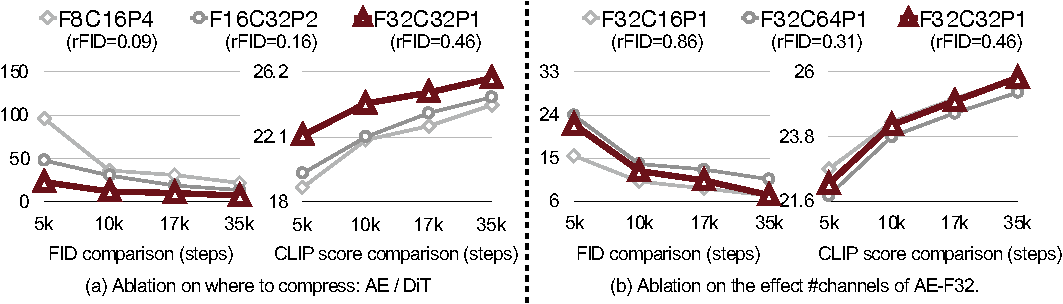
\includegraphics[width=0.90\textwidth]{figures/vae_ablation.pdf}
    \caption{
        Ablation study on our deep compression autoencoder (AE).
    }
    \label{fig:f8p4-f16p2-f32p1_2}
  \end{figure}


\noindent\textbf{Different Channels in AE-F32}: We explore various channel configurations and finally choose C=32 as our optimal setting. As shown in Figure~\ref{fig:f8p4-f16p2-f32p1_2}(b), fewer channels converge more quickly, but the reconstruction quality is worse. We observe that after 35K training steps, the convergence speeds of C=16 and C=32 are similar; however, C=32 yields better reconstruction metrics, resulting in better FID and CLIP scores. Although C=64 offers superior reconstruction, its following DiT's training convergence speed is significantly slower than that of C=32.


\begin{wrapfigure}{r}{0.5\columnwidth}
    \vspace{-2em}  % Moves the figure upwards relative to the surrounding text
    \centering
    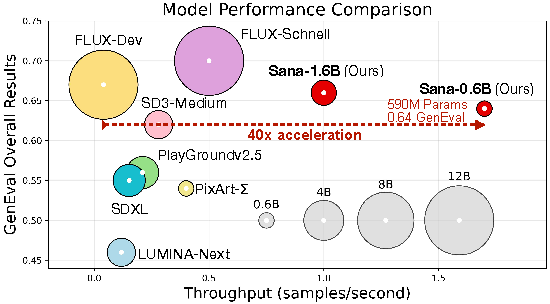
\includegraphics[width=0.99\linewidth]{figures/performance-bubble.pdf}
    \vspace{-1em}  % Reduces the space below the figure
    \caption{Comparison between \model and state-of-the-art diffusion models under 1024$\times$1024 resolution. All models are tested on an A100 GPU. 
    \model provides 0.64 GenEval overall performance with only 590M model parameters.
    }
    \label{fig:model_size}
    \vspace{-2em}  % Adjust this for controlling space after the figure
\end{wrapfigure}



\subsection{Efficient Linear DiT Design} \label{sec:efficient_design}

The self-attention used by DiT has a computational complexity of O(N$^2$), resulting in low computational efficiency when processing high-resolution images and incurring significant overhead. To address this issue, we first proposed linear DiT, which completely replaces the original self-attention with linear attention, achieving higher computational efficiency in high-resolution generation without compromising performance. In addition, we employ Mix-FFN to replace the original MLP-FFN, incorporating 3$\times$3 depth-wise convolution to better aggregate token information. These micro designs are inspired by \cite{cai2023efficientvit,xie2021segformer}, but we keep DiT's macro architecture design to maintain simplicity and scalability.

\begin{figure}[!ht]
    \centering
    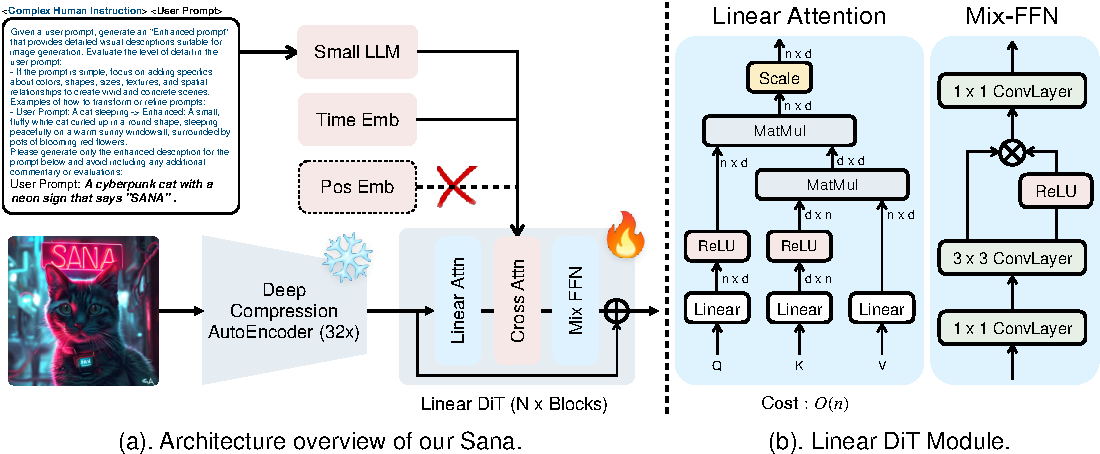
\includegraphics[width=0.99\linewidth]{figures/model.pdf}
    \vspace{-1mm}
    \caption{\textbf{Overview of \model}: Fig.~(a) describes the high-level training pipeline, containing our 32$\times$ deep compression Autoencoder, Linear DiT, and complex human instruction. Note that Positional embedding is not required in our framework. Fig.~(b) describes the detailed design of the Linear Attention and Mix-FFN in Linear DiT.  
    \vspace{-1em}
    }
    \label{fig:model_structure}
\end{figure}


\noindent \textbf{Linear Attention block.}
An illustration of our utilized linear attention module is provided in Figure~\ref{fig:model_structure}. 
To reduce computational complexity, we replace the traditional softmax attention with ReLU linear attention~\citep{katharopoulos2020transformers}. 
While ReLU linear attention and other variants~\citep{cai2023efficientvit,wang2020linformer,shen2021efficient,bolya2022hydra} have primarily been explored in high-resolution dense prediction tasks, 
our work represents an early exploration to demonstrate the effectiveness of linear attention in image generation. 

The computational benefits of our approach are evident in the implementation. As shown in Eq.~\ref{eq:relu_linear_attention}, instead of computing attention for each query, we compute shared terms \scalebox{0.8}{$\left( \sum_{j=1}^{N} \text{ReLU}(K_j)^T V_j \right) \in \mathbb{R}^{d \times d}$} and \scalebox{0.8}{$\left( \sum_{j=1}^{N} \text{ReLU}(K_j)^T \right) \in \mathbb{R}^{d \times 1}$} only once. These shared terms can then be reused for each query, leading to a linear computational complexity of $O(N)$ in both memory and computation.

\begin{equation}
  \vspace{-0.5em}
  \scalebox{1}{
    % O_i = \frac{\text{ReLU}(Q_i) \left( \sum_{j=1}^{N} \text{ReLU}(K_j)^T V_j \right)}{\text{ReLU}(Q_i) \left( \sum_{j=1}^{N} \text{ReLU}(K_j)^T \right)}.
    $O_i = \sum_{j=1}^{N} \frac{\text{ReLU}(Q_i) \text{ReLU}(K_j)^T V_j}{\sum_{j=1}^{N} \text{ReLU}(Q_i) \text{ReLU}(K_j)^T} = \frac{\text{ReLU}(Q_i) \left( \sum_{j=1}^{N} \text{ReLU}(K_j)^T V_j \right)}{\text{ReLU}(Q_i) \left( \sum_{j=1}^{N} \text{ReLU}(K_j)^T \right)}$
  }
  \label{eq:relu_linear_attention}
  \vspace{-0.5em}
\end{equation}

\noindent\textbf{Mix-FFN block.}
As discussed in EfficientViT~\citep{cai2023efficientvit}, linear attention models benefit from reduced computational complexity and lower latency compared to softmax attention. However, the absence of a non-linear similarity function may lead to sub-optimal performance. We observe a similar conclusion in image generation, where linear attention models suffer from much slower convergence despite eventually achieving comparable performance.
To further improve training efficiency, we replace the original MLP-FFN with Mix-FFN. The Mix-FFN consists of an inverted residual block, a 3$\times$3 depth-wise convolution, and a Gated Linear Unit (GLU)~\citep{dauphin2017language}. The depth-wise convolution enhances the model's ability to capture local information, compensating for the weaker local information-capturing ability of ReLU linear attention. Performance ablations for the model design space are shown in Table~\ref{tab:blocks_ablation}.

\noindent\textbf{DiT without Positional Encoding~(NoPE).} 
We are surprised that we can remove Positional Embedding without any loss in performance. Some earlier theoretical and practical works have mentioned that introducing 3$\times$3 convolution with zero padding can implicitly incorporate the position information~\citep{islam2020much,xie2021segformer}. 
In contrast to previous DiT-based methods that mostly use absolute PE, learnable PE, and RoPE, we propose NoPE, the first design that entirely omits positional embedding in DiT. Recent cutting-edge research in the LLM field~\citep{kazemnejad2024impact,haviv2022transformer} has also indicated that NoPE may offer better length generalization ability.


\noindent\textbf{Triton Acceleration Training/Inference.}
To further accelerate linear attention, we use Triton~\citep{tillet2019triton} to fuse kernels for both the forward and backward passes of the linear attention blocks to speed up training and inference.
By fusing all element-wise operations—including activation functions, precision conversions, padding operations, and divisions—into matrix multiplications, we reduce the overhead associated with data transfer. We attach more details and benefits coming from Triton to the appendix.


\subsection{Text Encoder Design} \label{sec:text_encoder}

\noindent \textbf{Why Replace T5 to Decoder-only LLM as Text Encoder? }
The most advanced LLMs nowadays are decoder-only GPT architectures that are trained on a larger scale of data. Compared to T5~(a method proposed in 2019), decoder-only LLMs possess powerful reasoning capabilities. They can follow complex human instructions by using Chain-of-Thought (CoT)~\citep{wei2022chain} and In-context-learning (ICL)~\citep{brown2020language}. 
In addition, some small LLMs, such as Gemma-2~\citep{team2024gemma2}, can rival the performance of large LLMs while being very efficient. Therefore, we choose to adopt Gemma-2 as our text encoder.

As shown in Table.~\ref{tab:text_encoder_comparison}, 
Compared to T5-XXL, Gemma-2-2B has an inference speed that is 6$\times$ faster, while the performance of Gemma-2B is comparable to T5-XXL in terms of Clip Score and FID.


\noindent \textbf{Stabilize Training using LLM as Text encoder:} We extract the last layer of features of the Gemma-2 decoder as text embedding. We empirically find that directly following the approach of using T5 text embedding as key, value, and image tokens (as the query) for cross-attention training results in extreme instability, with training loss frequently becoming NaN.

We find that the variance of T5's text embedding is several orders of magnitude smaller than that of the decoder-only LLMs~(Gemma-1-2B, Gemma-2-2B, Qwen-2-0.5B), indicating that there are many large absolute values in the text embedding output. To address this issue, we add a normalization layer (i.e., RMSNorm) after the decoder-only text encoder, which normalizes the variance of the text embeddings to 1.0. In addition, we discover a useful trick that further accelerates model convergence by initializing a small learnable scale factor (e.g., 0.01) and multiplying it by the text embedding. The results are shown in Figure~\ref{fig:ablation_y_norm_sf}.


\begin{figure}[h]
\centering
\begin{minipage}[t]{0.48\columnwidth}
  \centering
  \vspace{0pt}
    \captionof{table}{Ablation study of whether using \\Complex Human Instruction (CHI).}
    \vspace{-0.5em}
    \label{tab:ablation_chi}
    \scalebox{0.9}{
    \begin{tabular}{lll}
    \toprule
    \textbf{Prompt} & \textbf{Train Step} & \textbf{GenEval} \\
    \midrule
    User & \multirow{2}{*}{52K} & 45.5 \\
    CHI + User & & 47.7~(+2.2) \\
    \midrule
    User & 140K & 52.8 \\
    CHI + User & + 5K(finetune) & 54.8~(+2.0) \\
    \bottomrule
    \end{tabular}
    }
\end{minipage}
\hfill
\begin{minipage}[t]{0.48\columnwidth}
  \centering
  \vspace{0pt}
    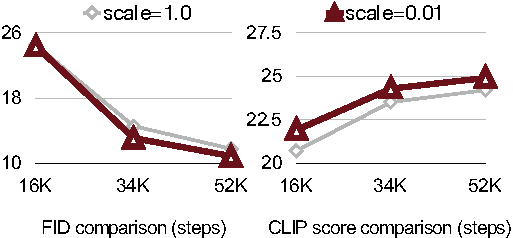
\includegraphics[width=0.9\textwidth]{figures/ablation_y_norm_scale_factor.pdf} 
    \vspace{-0.5em}
    \caption{Ablation study of whether using text embedding normalization and small scale factor. 
    }
    \label{fig:ablation_y_norm_sf}
\end{minipage}
\label{fig:combined}
\end{figure}

\begin{wrapfigure}{r}{0.5\columnwidth}
  \centering
  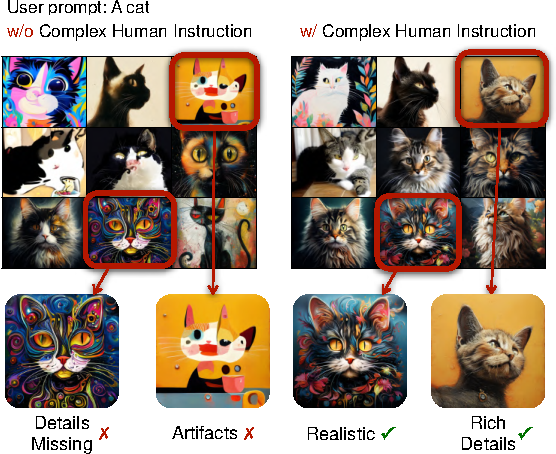
\includegraphics[width=0.99\linewidth]{figures/CHI.pdf}
  \caption{Generations w/ or w/o Complex-Human-Instruction (CHI). Without CHI, a simple prompt may lead to inferior generations, including artifacts and less-detailed results.}
  \label{fig:chi_visual}
  \vspace{-1.5em}
\end{wrapfigure}

\noindent \textbf{Complex Human Instruction Improves Text-Image Alignment:} As mentioned above, Gemma has better instruction-following capabilities than T5. We can further leverage this capability to strengthen text embedding. Gemma is a chat model, and although it possesses strong capabilities, it can be somehow unpredictable, thus we need to add instructions to help it focus on extracting and enhancing the prompt itself.
LiDiT~\citep{ma2024exploring} is the first to combine simple human instruction with user prompts. Here, we further expand it by using in-context learning of LLM to design a complex human instruction~(CHI). As shown in Table~\ref{tab:ablation_chi}, incorporating CHI during train—whether from scratch or through fine-tuning—can further improve the image-text alignment capability. 

Additionally, as shown in Figure~\ref{fig:chi_visual}, we find that when given a short prompt such as "a cat", CHI helps the model generate more stable content. This is evident in the fact that models without CHI often output content unrelated to the prompt.


\section{Efficient Training/Inference} \label{sec:efficient_train_infer}


\subsection{Data Curation and Blending} \label{data_curation}


\noindent \textbf{Multi-Caption Auto-labelling Pipeline:} 
For each image, whether or not it contains an original prompt, we will use four VLMs to label it: VILA-3B/13B~\citep{lin2024vila}, InternVL2-8B/26B~\citep{chen2024internvl}. Multiple VLMs can make the caption more accurate and more diverse. 

\noindent \textbf{CLIP-Score-based Caption Sampler:}
One problem multi-captioning presents is selecting the corresponding one for an image during training. The naive approach randomly selects a caption, which may select low-quality text and affect model performance.

We propose a clip score-based sampler, the motivation is to sample high-quality text with greater probability. We first calculate the clip score $c_i$ for all captions corresponding to an image, and then, when sampling, we sample according to the probability based on the clip score. Here, we introduce an additional hyper-parameter, temperature $\tau$, into the probability formulation \scalebox{0.8}{$P(c_i) = \frac{\exp\left(c_i / \tau\right)}{\sum_{j=1}^{N} \exp\left(c_j / \tau\right)}$}. The temperature can be used to adjust the sampling intensity. If the temperature is near 0, only the text with the highest clip score is sampled. The results in Table~\ref{tab:dataset_clip_ablation} show that variations in captions have minimal impact on image quality (FID) while improving semantic alignment during training.

\noindent \textbf{Cascade Resolution Training}: 
Benefiting from using AE-F32C32P1, we skip the 256px pre-training and start pre-training directly at a resolution of 512px, gradually fine-tuning the model to 1024px, 2K and 4K resolution.
We believe that the traditional practice of pre-training at 256px is too cost-effective, as images at 256 resolution lose too much detailed information, resulting in slower learning for the model in terms of image-text alignment.


\begin{figure}[h]
    \centering
    \begin{minipage}[t]{0.48\textwidth}
        \centering
        \vspace{0pt}
        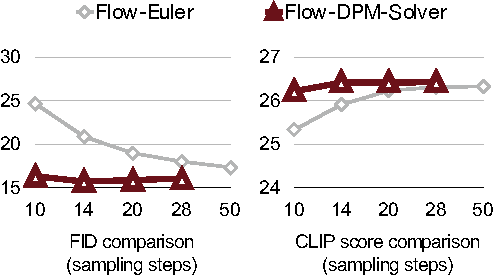
\includegraphics[width=1.0\linewidth]{figures/flow-sampler-ablation.pdf}
        \caption{Impact of sampling steps on FID and CLIP-Score: A Comparison between Flow-DPM-Solver and Flow-Euler.}
        \label{fig:flow_sampler_ablation}
    \end{minipage}
    \hfill
    \begin{minipage}[t]{0.48\textwidth}
        \centering
        \vspace{0pt}
        \captionof{table}{Comparison of different training schedules on 256$\times$256 resolution.}
        \label{tab:sampling_schedules}
        \vspace{-6pt}
        \scalebox{0.9}{
            \begin{tabular}{lccc}
                \toprule
                \textbf{Schedule} & \textbf{FID}~$\downarrow$ & \textbf{CLIP}~$\uparrow$ & \textbf{Iterations} \\
                \midrule
                DDPM & 19.5 & 24.6 & 120K \\
                Flow Matching & 16.9 & 25.7 & 120K \\
                \bottomrule
            \end{tabular}
        }
        
        \vspace{-5pt}
        \captionof{table}{Comparison of image-text pair sampling strategies during training.}
        \label{tab:dataset_clip_ablation}
        \vspace{2pt}
        \scalebox{0.9}{
            \begin{tabular}{lccc}
                \toprule
                \textbf{Prompt Strategy} & \textbf{FID}~$\downarrow$ & \textbf{CLIP}~$\uparrow$ & \textbf{Iterations} \\
                \midrule
                Single & 6.13 & 27.10 & 65K \\
                Multi-random & 6.15 & 27.13 & 65K \\
                Multi-clipscore & 6.12 & 27.26 & 65K \\
                \bottomrule
            \end{tabular}
        }
    \end{minipage}
\end{figure}

\subsection{Flow-based Training / Inference} \label{flow_schedule_train}

\noindent \textbf{Flow-based Training}: We analyze the superior performance of Rectified Flow from SD3~\citep{esser2024scaling} and find that, unlike DDPM~\citep{ho2020denoising}, which rely on noise prediction, both 1-Rectified Flow (RF)~\citep{lipman2022flow} and EDM~\citep{karras2022elucidating} use data or velocity prediction, resulting in faster convergence and improved performance. Specifically, all these methods follow a common diffusion formulation: $\mathbf{x}_t = \alpha_t \cdot \mathbf{x}_0 + \sigma_t \cdot \epsilon$, where $\mathbf{x}_0$ represents the image data, $\epsilon$ denotes random noise, and $\alpha_t$ and $\sigma_t$ are hyper-parameters of the diffusion process. In DDPM training, the objective is noise prediction, defined as $\epsilon_\theta(\mathbf{x}_t, t) = \epsilon_t$.
However, both EDM and RF follow a different approach: EDM aims for data prediction with the objective $x_\theta(\mathbf{x}_t, t) = \mathbf{x}_0$, while RF uses velocity prediction with the objective $v_\theta (\mathbf{x}_t, t) = \epsilon - \mathbf{x}_0$. 
This transition from noise prediction to data or velocity prediction is critical near $t = T$, where noise prediction can lead to instability, while data or velocity prediction provides more precise and stable estimates. As noted by \cite{balaji2022ediff}, attention activation near $t = T$ is stronger, further emphasizing the importance of accurate predictions at this critical point. This shift effectively reduces cumulative errors during sampling, resulting in faster convergence and improved performance. Further details can be found in Appendix~B.

\noindent \textbf{Flow-based Inference}: 
In our work, we modify the original DPM-Solver++~\citep{lu2022dpm_add} adapting the Rectified Flow formulation, named Flow-DPM-Solver. 
The key adjustments involve substituting the scaling factor $\alpha_t$ with $1 - \sigma_t$, where $\sigma_t$ remains unchanged but time-steps are redefined over the range $[0, 1]$ instead of $[1, 1000]$, 
with a time-step shift applied to achieve a lower signal-noise ratio, following SD3~\citep{esser2024scaling}. 
Additionally, our model predicts the velocity field, which differs from the data prediction in the original DPM-Solver++.
Specifically, data is derived from the relation: 
$\text{data} \gets x_0 = x_{T} - {\sigma}_{T} \cdot v_{\theta}(x_T, t_T)$,
where $v_\theta(\cdot)$ is the velocity predicted by the model.

As a result, in Figure~\ref{fig:flow_sampler_ablation}, our Flow-DPM-Solver converges at 14$\sim$20 steps with better performance, while the Flow-Euler sampler needs 28$\sim$50 steps for convergence with a worse result.


\section{On-device Deployment} \label{sec:deploy}

To enhance edge deployment, we quantize our model with 8-bit integers. Specifically, we adopt per-token symmetric INT8 quantization for activation and per-channel symmetric INT8 quantization for weights. Moreover, to preserve a high semantic similarity to the 16-bit variant while incurring minimal runtime overhead, we retain normalization layers, linear attention, and key-value projection layers within the cross-attention block at full precision.

\begin{table}[htbp]
\centering
\captionof{table}{\textbf{On-device Deployment}: our inference engine with W8A8 quantization realized a 2.4$\times$ speedup when generating 1024px images on the laptop GPU. The performance of \model{} is assessed with the CLIP-Score on MJHQ-30K~\citep{li2024playground} and the Image-Reward~\citep{xu2024imagereward} on its first 1K images.}
\vspace{-1em}
\label{table:quantization}
\scalebox{0.8}{
\begin{tabular}{lccc}
\toprule
\textbf{Methods} & \textbf{Latency~(s)} & \textbf{CLIP-Score}$~\uparrow$ & \textbf{Image-Reward}$~\uparrow$ \\
\midrule
\model~(FP16) & 0.88 & 28.5 & 1.03 \\
~~~~+ W8A8 Quantization & 0.37 & 28.3 & 0.96 \\
\bottomrule
\end{tabular}
}
\end{table}


We implement our W8A8 GEMM kernel in CUDA C++ and employ kernel fusion techniques to mitigate the overhead associated with unnecessary activation loads and stores, thereby enhancing overall performance. Specifically, we integrate the $\text{ReLU}(K)^TV$ product of linear attention (Equation~\ref{eq:relu_linear_attention}) with the $QKV$-projection layer; we also fuse the Gated Linear Unit (GLU) with the quantization kernel in Mix-FFN, and combine other element-wise operations. Additionally, we adjust the activation layout to avoid any transpose operations in GEMM and Conv kernels.

Table \ref{table:quantization} shows the speed comparison before and after our deployment optimization on a laptop GPU. For generating a 1024px image, our optimized implementation achieves 2.4$\times$ speedup, taking only 0.37 seconds, while maintaining almost lossless image quality.
